% --- IMPORTS ---
\documentclass[leqno]{article}
\usepackage{graphicx}
\usepackage{dsfont}
\usepackage{mathtools}
\usepackage{amssymb}
\usepackage{amsmath}
\usepackage{amsthm}
\usepackage{float}
\usepackage{ragged2e}
\usepackage{tensor}
\usepackage{fancyhdr}
\usepackage{empheq}
\usepackage[most]{tcolorbox}
\usepackage{enumitem}
\usepackage{dirtytalk}
\usepackage{marginnote}
\usepackage{microtype}
\usepackage[
  a4paper,
  left=0.8in,
  right=1in,
  top=1in,
  bottom=0.5in,
  headheight=14pt,
  headsep=0.4in
]{geometry}
\setlength{\parindent}{0cm}
% --- TikZ Packages ---
\usepackage{pgfplots}
\pgfplotsset{compat=1.18}
\usepgfplotslibrary{fillbetween, polar}
\usetikzlibrary{calc, positioning}
\usetikzlibrary{angles, quotes}
\usetikzlibrary{arrows.meta}
\usetikzlibrary{decorations.pathreplacing, decorations.markings}
\usetikzlibrary{patterns}
\usetikzlibrary{intersections}
% --- URL Packages ---
\usepackage[colorlinks=true,linkcolor=red,citecolor=magenta,urlcolor=black]{hyperref}%
\urlstyle{same}
% --- END OF IMPORTS ---

% --- CUSTOM COMMANDS ---
\RenewDocumentCommand{\marks}{o m}{%
  \IfValueTF{#1}%
    {\marginnote{\raggedright\textbf{[#2]}}[#1]}%
    {\marginnote{\raggedright\textbf{[#2]}}}%
}
\newcommand{\vspacerule}[2]{%
  \par\vspace*{#1}%
  \noindent\hrulefill\par
  \vspace*{#2}%
}
\definecolor{scarlet}{RGB}{205, 40, 75}
\newcommand{\questionitem}{%
  \item\phantomsection
  \addcontentsline{toc}{section}{Question \number\value{enumi}}%
}
\renewcommand{\contentsname}{Questions}
% --- END OF CUSTOM COMMANDS ---

% --- HEADER CONFIG ---
\pagestyle{fancy}
\fancyhead{}
\fancyfoot{}
\renewcommand{\headrulewidth}{0.9pt}
\lhead{\textit{Solutions} - Volumes of Revolution}
\chead{}
\rhead{\href{https://danieljsmith.org}{danieljsmith.org}}
% --- END OF HEADER CONFIG ---

\begin{document}
\vspace*{20pt}
\tableofcontents
\newpage
\begin{enumerate}[
  label=\textbf{\arabic*.},
  leftmargin=*,
  topsep=0pt,
  partopsep=0pt,
  parsep=0pt
]

% ---- Question 1 ----
\questionitem

\begin{figure}[H]
    \centering
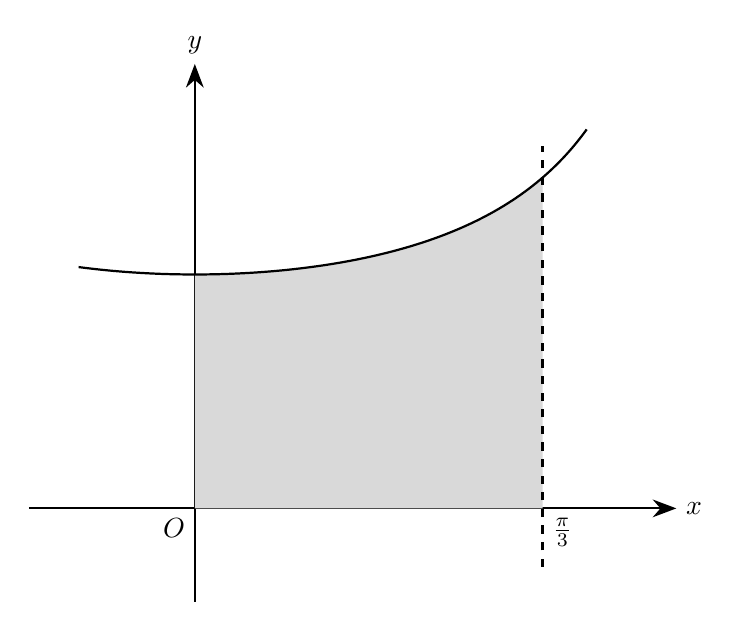
\begin{tikzpicture}[scale=1.2]
\def\xa{1.0472}
\begin{axis}[
    axis lines=middle,
    axis line style={-{Stealth[length=3mm]}, thick, black},
    xlabel={$x$},
    ylabel={$y$},
    xmin=-0.5, xmax=1.45,
    ymin=-0.4, ymax=1.9,
    xtick=\empty,
    ytick=\empty,
    clip=false,
    every axis x label/.style={at={(ticklabel* cs:1)}, anchor=west},
    every axis y label/.style={at={(ticklabel* cs:1)}, anchor=south}
]
\addplot[name path=curve, thick, black, samples=200, domain=-0.35:1.18] {sqrt(1/cos(deg(x)))};
\addplot[name path=xaxisline, draw=none, domain=0:\xa] {0};
\addplot[gray!30, draw=none] fill between[of=curve and xaxisline, soft clip={domain=0:\xa}];
\addplot[dashed, thick, black] coordinates {(\xa,-0.25) (\xa,1.55)};
\node[below left] at (axis cs:0,0) {$O$};
\node[below right] at (axis cs:\xa,0) {$\frac{\pi}{3}$};
\end{axis}
\end{tikzpicture}
\end{figure}


The shaded region is enclosed by the curve $y = \sqrt{\sec x}$, the coordinate axes and the line $x = \frac{\pi}{3}$. \\

The region is rotated completely about the $x$-axis. \\
Find the exact volume of the solid generated. \marks{3}

\vspace*{10pt}

\begin{tcolorbox}[colback=white, colframe=scarlet, title={\textbf{Solution}}, breakable, grow to left by=6mm, grow to right by=10mm]
Since the region is rotated about the $x$-axis, the volume is
\[
V=\pi\int_a^b y^2\,\mathrm{d}x
\]

Here the limits are $x=0$ to $x=\frac{\pi}{3}$, and
\[
y=\sqrt{\sec x}\implies y^2=\sec x
\]

So
\[
V=\pi\int_0^{\pi/3}\sec x\,\mathrm{d}x
\]

Using
\[
\int \sec x\,\mathrm{d}x=\ln|\sec x+\tan x|+C
\]

we get
\[
V=\pi\left[\ln(\sec x+\tan x)\right]_0^{\pi/3}
\]

Now substitute the limits:
\[
V=\pi\left(\ln\left(\sec\frac{\pi}{3}+\tan\frac{\pi}{3}\right)-\ln(\sec 0+\tan 0)\right)
\]

\[
\sec\frac{\pi}{3}=2,\qquad \tan\frac{\pi}{3}=\sqrt{3},\qquad \sec 0=1,\qquad \tan 0=0
\]

Hence
\[
V=\pi\left(\ln(2+\sqrt{3})-\ln 1\right)
\]

\[
V=\pi\ln(2+\sqrt{3})
\]

So the exact volume is $\pi\ln(2+\sqrt{3})$.
\end{tcolorbox}


\newpage

% ---- Question 2 ----
\questionitem

\begin{figure}[H]
    \centering
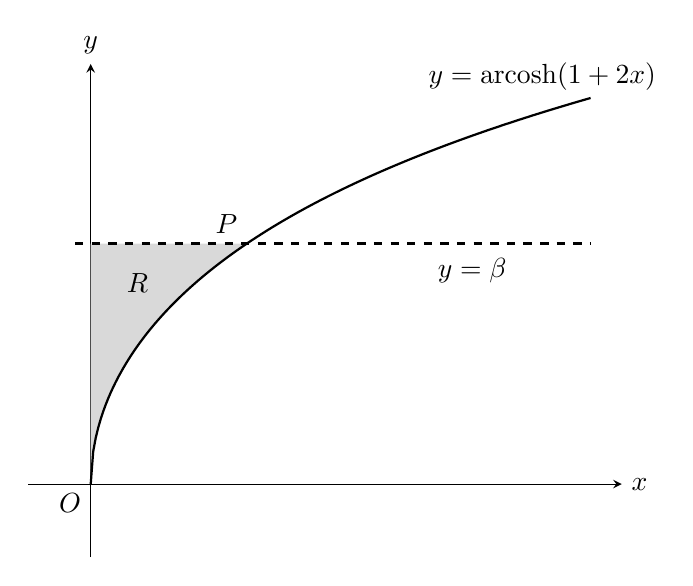
\begin{tikzpicture}[scale=1.1]
\pgfmathsetmacro{\betaval}{ln(2+sqrt(3))}
\pgfmathsetmacro{\alphaval}{1/2}
\begin{axis}[
    axis lines=center,
    xlabel={$x$},
    ylabel={$y$},
    xmin=-0.2, xmax=1.7,
    ymin=-0.4, ymax=2.3,
    xtick=\empty,
    ytick=\empty,
    clip=false,
    every axis x label/.style={at={(ticklabel* cs:1)}, anchor=west},
    every axis y label/.style={at={(ticklabel* cs:1)}, anchor=south},
]
\addplot[name path=lineclip, draw=none, domain=0:\alphaval] {\betaval};
\addplot[name path=curveclip, draw=none, samples=200, domain=0:\alphaval] {ln(1 + 2*x + sqrt((1 + 2*x)^2 - 1))};
\addplot[gray!30] fill between[of=lineclip and curveclip];
\addplot[thick, black, samples=200, domain=0:1.6] {ln(1 + 2*x + sqrt((1 + 2*x)^2 - 1))};
\addplot[thick, black, dashed, domain=-0.05:1.6] {\betaval};
\node[above right] at (axis cs:1.05,2.1) {$y=\operatorname{arcosh}(1+2x)$};
\node[right] at (axis cs:1.08,\betaval-0.15) {$y=\beta$};
\node at (axis cs:0.15,1.1) {$R$};
\node[below left] at (axis cs:0,0) {$O$};
\node[above left] at (axis cs:\alphaval,\betaval) {$P$};
\end{axis}
\end{tikzpicture}
\end{figure}


The diagram above shows a sketch of part of the curve with equation
\[
y = \operatorname{arcosh}(1 + 2x) \qquad x \geq 0
\] \\
and the straight line with equation $y = \beta$. \\

The line and the curve intersect at the point with coordinates $(\alpha, \beta)$. \\

Given that $\beta = \ln(2+\sqrt{3})$, \\

\begin{enumerate}[label=\textbf{(\alph*)}]
  \item show that $\alpha = \dfrac{1}{2}$. \marks{3} \\
\end{enumerate}
The finite region $R$, shown shaded in the diagram above, is bounded by the curve with equation $y = \operatorname{arcosh}(1 + 2x)$, the $y$-axis and the line with equation $y = \beta$. \\

  The region $R$ is rotated through $2\pi$ radians about the $y$-axis. \\
\begin{enumerate}[label=\textbf{(\alph*)}, resume]
\item Use calculus to find the exact value of the volume of the solid generated. \marks{6} \\
\end{enumerate}

\vspace*{10pt}

\begin{tcolorbox}[colback=white, colframe=scarlet, title={\textbf{Solution}}, breakable, grow to left by=6mm, grow to right by=10mm]
\begin{enumerate}[label=\textbf{(\alph*)}]
  \item At the point of intersection, $(\alpha,\beta)$ lies on the curve
\[
y=\operatorname{arcosh}(1+2x)
\]
so
\[
\beta=\operatorname{arcosh}(1+2\alpha)
\]
Applying $\cosh$ to both sides gives
\[
\cosh\beta=1+2\alpha
\]

Given
\[
\beta=\ln(2+\sqrt3)
\]
and using
\[
\operatorname{arcosh}2=\ln(2+\sqrt{2^2-1})=\ln(2+\sqrt3)
\]
we have
\[
\beta=\operatorname{arcosh}2
\]
so
\[
\cosh\beta=2
\]

Therefore
\[
1+2\alpha=2
\]
and hence
\[
2\alpha=1
\]
so
\[
\alpha=\frac12
\]

So the required value is $\alpha=\frac12$.

  \item First write $x$ in terms of $y$.

From
\[
y=\operatorname{arcosh}(1+2x)
\]
we get
\[
\cosh y=1+2x
\]
so
\[
x=\frac{\cosh y-1}{2}
\]

When $x=0$,
\[
y=\operatorname{arcosh}(1)=0
\]
and the top of the region is $y=\beta$. Hence $0\le y\le \beta$.

When the region is rotated about the $y$-axis, the volume is
\[
V=\pi\int_0^\beta x^2\,\mathrm{d}y
\]
So
\[
V=\pi\int_0^\beta \left(\frac{\cosh y-1}{2}\right)^2\,\mathrm{d}y
=\frac{\pi}{4}\int_0^\beta (\cosh y-1)^2\,\mathrm{d}y
\]

Now expand:
\begin{align*}
(\cosh y-1)^2
&=\cosh^2 y-2\cosh y+1
\end{align*}
and use
\[
\cosh^2 y=\frac{\cosh 2y+1}{2}
\]
to get
\begin{align*}
(\cosh y-1)^2
&=\frac{\cosh 2y+1}{2}-2\cosh y+1 \\
&=\frac12\cosh 2y-2\cosh y+\frac32
\end{align*}

Therefore
\begin{align*}
V
&=\frac{\pi}{4}\int_0^\beta \left(\frac12\cosh 2y-2\cosh y+\frac32\right)\,\mathrm{d}y \\
&=\frac{\pi}{4}\left[\frac14\sinh 2y-2\sinh y+\frac32 y\right]_0^\beta
\end{align*}

Now use the result from part (a), or equivalently $\beta=\operatorname{arcosh}2$, so
\[
\cosh\beta=2
\]
Hence
\[
\sinh\beta=\sqrt{\cosh^2\beta-1}=\sqrt{4-1}=\sqrt3
\]
since $\beta>0$.

Also,
\[
\sinh 2\beta=2\sinh\beta\cosh\beta=2(\sqrt3)(2)=4\sqrt3
\]

Substituting:
\begin{align*}
V
&=\frac{\pi}{4}\left[\frac14(4\sqrt3)-2(\sqrt3)+\frac32\beta\right] \\
&=\frac{\pi}{4}\left(\sqrt3-2\sqrt3+\frac32\beta\right) \\
&=\frac{\pi}{4}\left(-\sqrt3+\frac32\beta\right) \\
&=\frac{\pi}{8}(3\beta-2\sqrt3)
\end{align*}

Finally, since $\beta=\ln(2+\sqrt3)$,
\[
V=\frac{\pi}{8}\left(3\ln(2+\sqrt3)-2\sqrt3\right)
\]

So the exact volume is
\[
\frac{\pi}{8}\left(3\ln(2+\sqrt3)-2\sqrt3\right)
\]
\end{enumerate}
\end{tcolorbox}


\newpage

% ---- Question 3 ----
\questionitem

The equation of a curve is
\[
y = \sqrt{\frac{k-x}{k+x}}
\]
where $k$ is a positive constant. The region enclosed by the curve, the $x$-axis, the $y$-axis and the line $x = k$ is rotated through $2\pi$ radians about the $x$-axis. \\

Given that the volume of the solid of revolution formed is $1$ unit$^3$, find the exact value of $k$. \marks{4}

\vspace*{10pt}

\begin{tcolorbox}[colback=white, colframe=scarlet, title={\textbf{Solution}}, breakable, grow to left by=6mm, grow to right by=10mm]
When the region is rotated about the $x$-axis, the volume is given by
\[
V=\pi\int_0^k y^2\,\mathrm{d}x
\]

Here
\[
y=\sqrt{\frac{k-x}{k+x}}
\]
so
\[
y^2=\frac{k-x}{k+x}
\]

Given that the volume is $1\text{ unit}^3$,
\[
1=\pi\int_0^k \frac{k-x}{k+x}\,\mathrm{d}x
\]

First simplify the integrand:
\[
\frac{k-x}{k+x}=\frac{-(k+x)+2k}{k+x}=-1+\frac{2k}{k+x}
\]

So
\begin{align*}
1&=\pi\int_0^k \left(-1+\frac{2k}{k+x}\right)\,\mathrm{d}x \\
&=\pi\left[\,-x+2k\ln(k+x)\right]_0^k \\
&=\pi\left(\left[-k+2k\ln(2k)\right]-\left[0+2k\ln k\right]\right) \\
&=\pi\left(-k+2k\bigl(\ln(2k)-\ln k\bigr)\right) \\
&=\pi\left(-k+2k\ln 2\right) \\
&=\pi k(2\ln 2-1)
\end{align*}

Hence
\[
k=\frac{1}{\pi(2\ln 2-1)}
\]

Therefore, the exact value of $k$ is
\[
\frac{1}{\pi(2\ln 2-1)}
\]
\end{tcolorbox}


\newpage

% ---- Question 4 ----
\questionitem

\begin{enumerate}[label=\textbf{(\alph*)}]
  \item Find
  \[
  \int \sin^2\theta\,\mathrm{d}\theta
  \]
  \marks[-20pt]{2}
\end{enumerate}

\begin{figure}[H]
    \centering
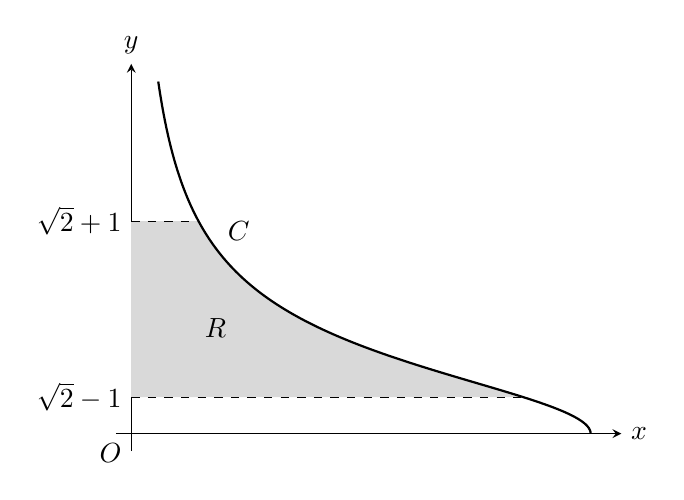
\begin{tikzpicture}
\pgfmathsetmacro{\ya}{sqrt(2)-1}
\pgfmathsetmacro{\yb}{sqrt(2)+1}
\pgfmathsetmacro{\xa}{6/(1+\ya*\ya)}
\pgfmathsetmacro{\xb}{6/(1+\yb*\yb)}
\begin{axis}[
    axis lines=center,
    xlabel={$x$},
    ylabel={$y$},
    xmin=-0.2, xmax=6.4,
    ymin=-0.2, ymax=4.2,
    xtick=\empty,
    ytick=\empty,
    width=8cm,
    height=6.5cm,
    clip=false,
    every axis x label/.style={at={(ticklabel* cs:1)}, anchor=west},
    every axis y label/.style={at={(ticklabel* cs:1)}, anchor=south}
]

\path[fill=gray!30]
    (axis cs:0,\ya) --
    (axis cs:0,\yb) --
    plot[domain=\yb:\ya, samples=200, variable=\u]
        (axis cs:{6/(1+\u^2)},{\u})
    -- cycle;

\addplot[thick, black, samples=200, domain=0:4, variable=\u]
    ({6/(1+\u^2)}, {\u})
    node[pos=0.72, above right] {$C$};

\addplot[dashed, black] coordinates {(0,\ya) (\xa,\ya)};
\addplot[dashed, black] coordinates {(0,\yb) (\xb,\yb)};

\node[below left] at (axis cs:0,0) {$O$};
\node[left] at (axis cs:0,\ya) {$\sqrt{2}-1$};
\node[left] at (axis cs:0,\yb) {$\sqrt{2}+1$};
\node at (axis cs:1.1,1.2) {$R$};

\end{axis}
\end{tikzpicture}
\end{figure}


The diagram shows part of the curve $C$ with parametric equations $x=6\sin^2\theta$, $y=\cot\theta$, $0<\theta\leq\frac{\pi}{2}$. \\

The finite region $R$ shown in the diagram is bounded by $C$, the lines $y=\sqrt{2}-1$, $y=\sqrt{2}+1$ and the $y$-axis. Region $R$ is rotated through $2\pi$ radians about the $y$-axis to form a solid of revolution. \\
\begin{enumerate}[label=\textbf{(\alph*)}, resume]
  \item Show that the volume of the solid of revolution formed is given by the integral
  \[
  k\int_a^b \sin^2\theta\,\mathrm{d}\theta
  \]
  where $a$, $b$ and $k$ are constants to be found. \marks{5} \\


\item Hence find the exact value of this volume, giving your answer in the form $p\pi^2$, where $p$ is a constant to be found. \marks{3} \\
\end{enumerate}

\vspace*{10pt}

\begin{tcolorbox}[colback=white, colframe=scarlet, title={\textbf{Solution}}, breakable, grow to left by=6mm, grow to right by=10mm]
\begin{enumerate}[label=\textbf{(\alph*)}]
  \item Use the identity
  \[
  \sin^2\theta=\frac{1-\cos 2\theta}{2}
  \]
  Then
  \begin{align*}
  \int \sin^2\theta\,\mathrm{d}\theta
  &= \int \frac{1-\cos 2\theta}{2}\,\mathrm{d}\theta \\
  &= \frac12\int 1\,\mathrm{d}\theta-\frac12\int \cos 2\theta\,\mathrm{d}\theta \\
  &= \frac{\theta}{2}-\frac12\cdot\frac{\sin 2\theta}{2}+C \\
  &= \frac{\theta}{2}-\frac{\sin 2\theta}{4}+C
  \end{align*}
  Hence
  \[
  \int \sin^2\theta\,\mathrm{d}\theta=\frac{\theta}{2}-\frac{\sin 2\theta}{4}+C
  \]

  \item When the region is rotated about the $y$-axis, the volume is
  \[
  V=\pi\int x^2\,\mathrm{d}y
  \]
  Here
  \[
  x=6\sin^2\theta,\qquad y=\cot\theta
  \]
  so
  \[
  \frac{\mathrm{d}y}{\mathrm{d}\theta}=-\operatorname{cosec}^2\theta
  \]

  We now find the $\theta$-limits.

  When $y=\sqrt2+1$,
  \[
  \cot\theta=\sqrt2+1
  \]
  and since $\tan\frac{\pi}{8}=\sqrt2-1$, it follows that
  \[
  \cot\frac{\pi}{8}=\sqrt2+1
  \]
  so $\theta=\frac{\pi}{8}$.

  When $y=\sqrt2-1$,
  \[
  \cot\theta=\sqrt2-1
  \]
  and
  \[
  \cot\frac{3\pi}{8}=\tan\frac{\pi}{8}=\sqrt2-1
  \]
  so $\theta=\frac{3\pi}{8}$.

  Therefore
  \begin{align*}
  V
  &=\pi\int_{\sqrt2-1}^{\sqrt2+1} x^2\,\mathrm{d}y \\
  &=\pi\int_{3\pi/8}^{\pi/8} (6\sin^2\theta)^2\frac{\mathrm{d}y}{\mathrm{d}\theta}\,\mathrm{d}\theta \\
  &=\pi\int_{3\pi/8}^{\pi/8} (6\sin^2\theta)^2(-\operatorname{cosec}^2\theta)\,\mathrm{d}\theta \\
  &=36\pi\int_{3\pi/8}^{\pi/8} -\sin^2\theta\,\mathrm{d}\theta \\
  &=36\pi\int_{\pi/8}^{3\pi/8} \sin^2\theta\,\mathrm{d}\theta
  \end{align*}

  So the required form is
  \[
  k\int_a^b \sin^2\theta\,\mathrm{d}\theta
  \]
  with
  \[
  k=36\pi,\qquad a=\frac{\pi}{8},\qquad b=\frac{3\pi}{8}
  \]

  \item Using parts (a) and (b),
  \begin{align*}
  V
  &=36\pi\int_{\pi/8}^{3\pi/8}\sin^2\theta\,\mathrm{d}\theta \\
  &=36\pi\left[\frac{\theta}{2}-\frac{\sin 2\theta}{4}\right]_{\pi/8}^{3\pi/8} \\
  &=36\pi\left(\frac{3\pi}{16}-\frac{\sin(3\pi/4)}{4}-\frac{\pi}{16}+\frac{\sin(\pi/4)}{4}\right)
  \end{align*}

  Since
  \[
  \sin\frac{3\pi}{4}=\sin\frac{\pi}{4}
  \]
  the sine terms cancel, giving
  \begin{align*}
  V
  &=36\pi\left(\frac{2\pi}{16}\right) \\
  &=36\pi\cdot\frac{\pi}{8} \\
  &=\frac{9\pi^2}{2}
  \end{align*}

  Hence the exact volume is
  \[
  \frac{9\pi^2}{2}
  \]
  so $p=\frac92$.
\end{enumerate}
\end{tcolorbox}


\newpage

% ---- Question 5 ----
\questionitem

\begin{enumerate}[label=\textbf{(\alph*)}]
  \item Show that $\sinh(2\ln 2)=\frac{15}{8}$. \marks{2} \\
\end{enumerate}

\begin{figure}[H]
    \centering
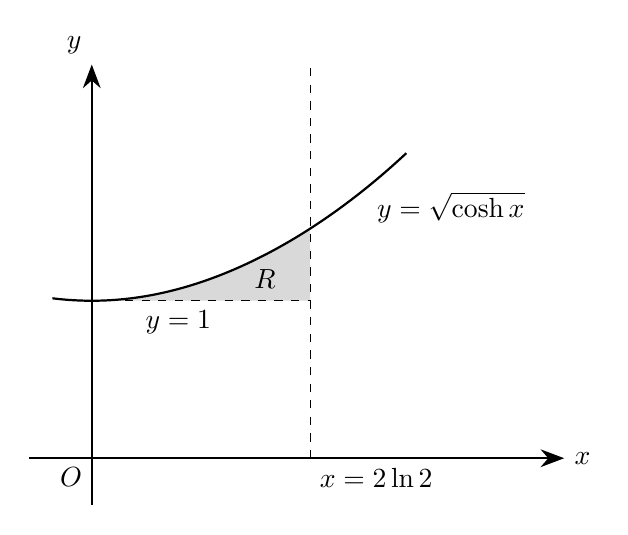
\begin{tikzpicture}[scale=2]
\def\xmin{-0.4}
\def\xmax{3}
\def\ymin{-0.3}
\def\ymax{2.5}
\def\xv{1.386294361}

\draw[-{Stealth[length=3mm]}, thick] (\xmin,0) -- (\xmax,0) node[right] {$x$};
\draw[-{Stealth[length=3mm]}, thick] (0,\ymin) -- (0,\ymax) node[above left] {$y$};

\fill[gray!30] (0,1) --
  plot[domain=0:\xv, samples=200] (\x, {sqrt((exp(\x)+exp(-\x))/2)}) --
  (\xv,1) -- cycle;

\draw[thick, domain=-0.25:2.0, samples=200] plot (\x, {sqrt((exp(\x)+exp(-\x))/2)});
\draw[dashed] (0,1) -- (\xv,1);
\draw[dashed] (\xv,0) -- (\xv,\ymax);

\node[below left] at (0,0) {$O$};
\node at (1.1,1.14) {$R$};
\node[above right] at (1.75,1.43) {$y=\sqrt{\cosh x}$};
\node[below right] at (0.28,1) {$y=1$};
\node[below right] at (\xv,0) {$x=2\ln 2$};
\end{tikzpicture}
\end{figure}


The region $R$ is bounded by the curve with equation $y=\sqrt{\cosh x}$, the line $y=1$ and the line $x=2\ln 2$, as shown in the diagram. The units of the axes are centimetres. \\

A designer models a hollow glass ornament as the solid formed by rotating $R$ completely about the $x$-axis. \\
\begin{enumerate}[label=\textbf{(\alph*)}, resume]
  \item Determine, according to the model, the exact volume of the ornament. \marks{4} \\
\end{enumerate}

\vspace*{10pt}

\begin{tcolorbox}[colback=white, colframe=scarlet, title={\textbf{Solution}}, breakable, grow to left by=6mm, grow to right by=10mm]
\begin{enumerate}[label=\textbf{(\alph*)}]
  \item Using
  \[
  \sinh u=\frac{e^u-e^{-u}}{2}
  \]
  with $u=2\ln 2$,
  \begin{align*}
  \sinh(2\ln 2)
  &=\frac{e^{2\ln 2}-e^{-2\ln 2}}{2} \\
  &=\frac{e^{\ln 4}-e^{-\ln 4}}{2} \\
  &=\frac{4-\frac14}{2} \\
  &=\frac{\frac{16}{4}-\frac14}{2}
   =\frac{15/4}{2}
   =\frac{15}{8}
  \end{align*}
  Hence,
  \[
  \sinh(2\ln 2)=\frac{15}{8}
  \]

  \item First find the left-hand limit of the region by solving where the curve meets $y=1$:
  \begin{align*}
  \sqrt{\cosh x} &= 1 \\
  \cosh x &= 1
  \end{align*}
  and this gives $x=0$.

  So the region extends from $x=0$ to $x=2\ln 2$.

  When the region is rotated about the $x$-axis, the volume is
  \[
  V=\pi\int_a^b \left((\text{upper curve})^2-(\text{lower curve})^2\right)\,\mathrm{d}x
  \]
  Here, the upper curve is $y=\sqrt{\cosh x}$ and the lower curve is $y=1$, so
  \begin{align*}
  V&=\pi\int_0^{2\ln 2}\left(\left(\sqrt{\cosh x}\right)^2-1^2\right)\,\mathrm{d}x \\
   &=\pi\int_0^{2\ln 2}(\cosh x-1)\,\mathrm{d}x
  \end{align*}

  Integrating,
  \begin{align*}
  V&=\pi\left[\sinh x-x\right]_0^{2\ln 2} \\
   &=\pi\left(\sinh(2\ln 2)-2\ln 2-(\sinh 0-0)\right) \\
   &=\pi\left(\sinh(2\ln 2)-2\ln 2\right)
  \end{align*}

  From part (a), $\sinh(2\ln 2)=\dfrac{15}{8}$, so
  \[
  V=\pi\left(\frac{15}{8}-2\ln 2\right)\text{ cm}^3
  \]

  Therefore, the exact volume of the ornament is
  \[
  \pi\left(\frac{15}{8}-2\ln 2\right)\text{ cm}^3
  \]
\end{enumerate}
\end{tcolorbox}


\newpage

% ---- Question 6 ----
\questionitem

\begin{figure}[H]
    \centering
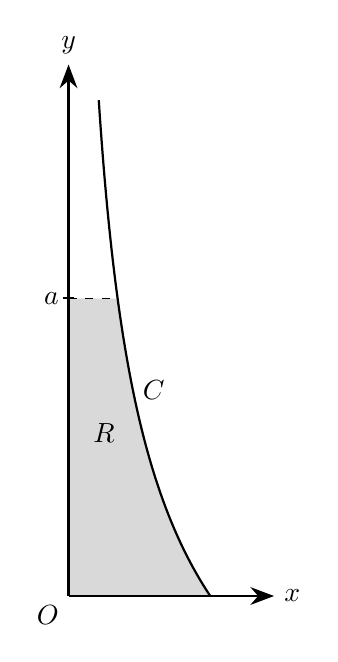
\begin{tikzpicture}[scale=1.8]
\def\a{2.1}
\def\ytop{3.5}
\def\xmax{1.45}
\def\ymax{3.75}
    \pgfmathsetmacro{\bx}{9/((\a+3)^2)}
\coordinate (O) at (0,0);
\coordinate (A) at (0,\a);
\coordinate (B) at (\bx,\a);
\coordinate (X) at (1,0);
\coordinate (RLab) at (0.25,1.15);
\coordinate (CLab) at ({9/((1.45+3)^2)},1.45);

\fill[gray!30] (O) -- (X) --
  plot[domain=0:\a, samples=200, variable=\yy] ({9/((\yy+3)^2)}, {\yy})
  -- (A) -- cycle;

\draw[thick, -{Stealth[length=3mm]}] (0,0) -- (\xmax,0) node[right] {$x$};
\draw[thick, -{Stealth[length=3mm]}] (0,0) -- (0,\ymax) node[above] {$y$};

\draw[thick] plot[domain=0:\ytop, samples=200, variable=\yy] ({9/((\yy+3)^2)}, {\yy});
\draw[dashed] (A) -- (B);

\draw[thick] (-0.04,\a) -- (0.04,\a);
\node[left] at (0,\a) {$a$};

\node[below left] at (O) {$O$};
\node at (RLab) {$R$};
\node[right] at (CLab) {$C$};
\end{tikzpicture}
\end{figure}


The curve $C$ is given parametrically by
\[
x = \frac{9}{t^4}, \qquad y = t^2 - 3, \qquad t \geq \sqrt{3}
\]
The shaded region $R$, shown in the diagram, is enclosed by $C$, the $x$-axis, the $y$-axis and the line $y=a$. When $R$ is rotated through $2\pi$ radians about the $y$-axis, the resulting solid has volume
\[
\frac{7\pi}{8}
\]
Find the exact value of $a$. \marks{8}

\vspace*{10pt}

\begin{tcolorbox}[colback=white, colframe=scarlet, title={\textbf{Solution}}, breakable, grow to left by=6mm, grow to right by=10mm]
First write the curve in the form \(x\) as a function of \(y\).

From
\[
y=t^2-3
\]
we have
\[
t^2=y+3
\]
So
\[
x=\frac{9}{t^4}=\frac{9}{(t^2)^2}=\frac{9}{(y+3)^2}
\]

Since \(t\ge \sqrt{3}\), we have \(y\ge 0\), so the region runs from \(y=0\) up to \(y=a\).

When the region is rotated about the \(y\)-axis, the volume is
\[
V=\pi\int_0^a x^2\,\mathrm{d}y
\]
Hence
\begin{align*}
V&=\pi\int_0^a \left(\frac{9}{(y+3)^2}\right)^2\,\mathrm{d}y\\
&=\pi\int_0^a \frac{81}{(y+3)^4}\,\mathrm{d}y\\
&=81\pi\int_0^a (y+3)^{-4}\,\mathrm{d}y\\
&=81\pi\left[\frac{(y+3)^{-3}}{-3}\right]_0^a\\
&=81\pi\left[-\frac{1}{3(y+3)^3}\right]_0^a\\
&=81\pi\left(-\frac{1}{3(a+3)^3}+\frac{1}{3\cdot 3^3}\right)\\
&=81\pi\left(-\frac{1}{3(a+3)^3}+\frac{1}{81}\right)\\
&=-\frac{27\pi}{(a+3)^3}+\pi\\
&=\pi\left(1-\frac{27}{(a+3)^3}\right)
\end{align*}

We are told that the volume is \(\dfrac{7\pi}{8}\), so
\begin{align*}
\pi\left(1-\frac{27}{(a+3)^3}\right)&=\frac{7\pi}{8}\\
1-\frac{27}{(a+3)^3}&=\frac{7}{8}\\
\frac{27}{(a+3)^3}&=\frac{1}{8}\\
(a+3)^3&=216
\end{align*}

Now \(a\ge 0\), so \(a+3>0\), and therefore
\[
a+3=6
\]
Thus
\[
a=3
\]

The exact value of \(a\) is \(3\).
\end{tcolorbox}


\newpage

% ---- Question 7 ----
\questionitem

\begin{figure}[H]
    \centering
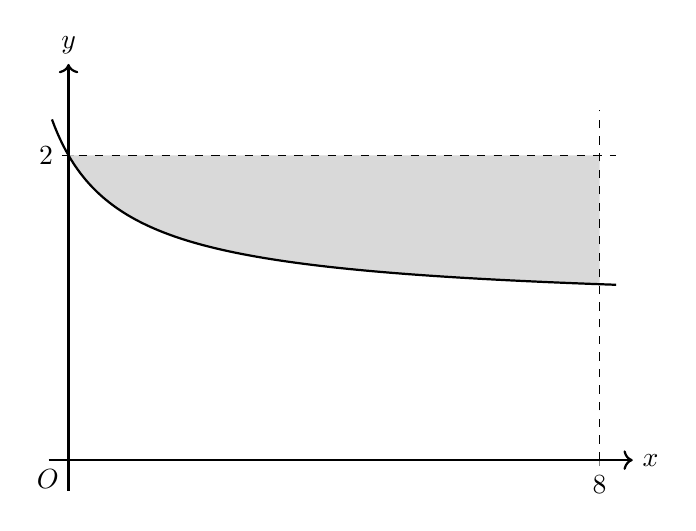
\begin{tikzpicture}
\begin{axis}[
    axis lines=middle,
    axis line style={->, thick},
    xlabel={$x$},
    ylabel={$y$},
    xmin=-0.3, xmax=8.5,
    ymin=-0.2, ymax=2.6,
    xtick={8},
    ytick={2},
    xticklabels={$8$},
    yticklabels={$2$},
    width=9cm,
    height=7cm,
    clip=false,
    every axis x label/.style={at={(ticklabel* cs:1)}, anchor=west},
    every axis y label/.style={at={(ticklabel* cs:1)}, anchor=south}
]
\addplot[name path=top, draw=none, domain=0:8, samples=2] {2};
\addplot[name path=curvefill, draw=none, domain=0:8, samples=200] {sqrt((x+4)/(x+1))};
\addplot[gray!30] fill between[of=top and curvefill];

\addplot[thick, black, domain=-0.25:8.25, samples=200] {sqrt((x+4)/(x+1))};
\addplot[dashed, black, domain=-0.1:8.25, samples=2] {2};
\addplot[dashed, black] coordinates {(8,0) (8,2.3)};

\node[below left] at (axis cs:0,0) {$O$};
\end{axis}
\end{tikzpicture}
\end{figure}


The diagram shows the region bounded by the curve $y = \sqrt{\dfrac{x+4}{x+1}}$, the line $y = 2$ and the line $x = 8$. The curve meets the line $y = 2$ at the point $(0,2)$. \\

Find the exact volume of the solid formed when this region is rotated through $360^\circ$ about the $x$-axis. \marks{6}

\vspace*{10pt}

\begin{tcolorbox}[colback=white, colframe=scarlet, title={\textbf{Solution}}, breakable, grow to left by=6mm, grow to right by=10mm]
The region is between the line $y=2$ and the curve
\[
y=\sqrt{\frac{x+4}{x+1}}
\]
from $x=0$ to $x=8$.

When this region is rotated about the $x$-axis, the volume is
\[
V=\pi\int_0^8 \left(2^2-\left(\sqrt{\frac{x+4}{x+1}}\right)^2\right)\,\mathrm{d}x
\]

So
\[
V=\pi\int_0^8\left(4-\frac{x+4}{x+1}\right)\,\mathrm{d}x
\]

Simplify the integrand:
\begin{align*}
4-\frac{x+4}{x+1}
&=\frac{4(x+1)-(x+4)}{x+1} \\
&=\frac{4x+4-x-4}{x+1} \\
&=\frac{3x}{x+1}
\end{align*}

Hence
\[
V=\pi\int_0^8 \frac{3x}{x+1}\,\mathrm{d}x
=3\pi\int_0^8 \frac{x}{x+1}\,\mathrm{d}x
\]

Now write
\[
\frac{x}{x+1}=1-\frac{1}{x+1}
\]

Therefore
\[
V=3\pi\int_0^8\left(1-\frac{1}{x+1}\right)\,\mathrm{d}x
\]

Integrating gives
\[
V=3\pi\left[x-\ln(x+1)\right]_0^8
\]

Substitute the limits:
\begin{align*}
V&=3\pi\left((8-\ln 9)-(0-\ln 1)\right) \\
&=3\pi(8-\ln 9)
\end{align*}

Since $\ln 9=2\ln 3$,
\begin{align*}
V&=24\pi-3\pi\ln 9 \\
&=24\pi-6\pi\ln 3 \\
&=6\pi(4-\ln 3)
\end{align*}

So the exact volume is $6\pi(4-\ln 3)$.
\end{tcolorbox}


\newpage

% ---- Question 8 ----
\questionitem

The region in the first quadrant bounded by the curve $y = \sinh x$, the $y$-axis, and the line $y = 2$ is rotated through $360^\circ$ about the $x$-axis. \\

Find the exact volume of revolution generated, expressing your answer in a form involving a logarithm. \marks{7}

\vspace*{10pt}

\begin{tcolorbox}[colback=white, colframe=scarlet, title={\textbf{Solution}}, breakable, grow to left by=6mm, grow to right by=10mm]
Let the curve $y=\sinh x$ meet the line $y=2$ at $x=a$.

Then
\[
\sinh a=2
\]

To find $a$ in logarithmic form,
\begin{align*}
\sinh a=2
&\implies \frac{e^a-e^{-a}}{2}=2\\
&\implies e^a-e^{-a}=4\\
&\implies e^{2a}-1=4e^a
\end{align*}

Let $u=e^a$. Then $u>0$ and
\[
u^2-4u-1=0
\]

So
\[
u=\frac{4\pm\sqrt{16+4}}{2}=2\pm\sqrt{5}
\]

Since $u>0$, we take
\[
u=2+\sqrt5
\]

Hence
\[
a=\ln(2+\sqrt5)
\]

For $0\le x\le a$, the region lies between $y=\sinh x$ and $y=2$.  
When it is rotated about the $x$-axis, the volume is
\[
V=\pi\int_0^a \left(2^2-(\sinh x)^2\right)\,\mathrm{d}x
\]

So
\[
V=\pi\int_0^a \left(4-\sinh^2 x\right)\,\mathrm{d}x
\]

Use
\[
\sinh^2 x=\frac{\cosh 2x-1}{2}
\]

Then
\begin{align*}
V
&=\pi\int_0^a \left(4-\frac{\cosh 2x-1}{2}\right)\,\mathrm{d}x\\
&=\pi\int_0^a \left(\frac92-\frac12\cosh 2x\right)\,\mathrm{d}x\\
&=\pi\left[\frac92x-\frac14\sinh 2x\right]_0^a
\end{align*}

Now $\sinh a=2$, and since $a>0$,
\[
\cosh a=\sqrt{1+\sinh^2 a}=\sqrt{1+4}=\sqrt5
\]

Therefore
\[
\sinh 2a=2\sinh a\cosh a=2(2)(\sqrt5)=4\sqrt5
\]

Substituting into the volume,
\begin{align*}
V
&=\pi\left(\frac92a-\frac14\sinh 2a\right)\\
&=\pi\left(\frac92a-\frac14(4\sqrt5)\right)\\
&=\pi\left(\frac92a-\sqrt5\right)
\end{align*}

Finally, using $a=\ln(2+\sqrt5)$,
\[
V=\pi\left(\frac92\ln(2+\sqrt5)-\sqrt5\right)
\]

So the exact volume is
\[
\pi\left(\frac92\ln(2+\sqrt5)-\sqrt5\right)
\]
\end{tcolorbox}


\newpage

% ---- Question 9 ----
\questionitem

\begin{figure}[H]
    \centering
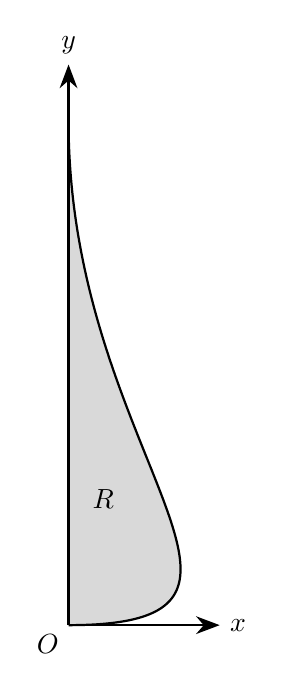
\begin{tikzpicture}[scale=0.8]
\def\tmax{1}
\def\xmax{2.4}
\def\ymax{8.9}

\fill[gray!30] (0,0)
  plot[samples=200,domain=0:\tmax,smooth,variable=\t] ({12*\t*(1-\t)*(1-\t)},{8*\t*\t}) -- cycle;

\draw[thick,-{Stealth[length=3mm]}] (0,0) -- (\xmax,0) node[right] {$x$};
\draw[thick,-{Stealth[length=3mm]}] (0,0) -- (0,\ymax) node[above] {$y$};
\draw[thick,samples=200,domain=0:\tmax,smooth,variable=\t] plot ({12*\t*(1-\t)*(1-\t)},{8*\t*\t});

\node[below left] at (0,0) {$O$};
\node at (0.55,2) {$R$};
\end{tikzpicture}
\end{figure}


Part of the side profile of a solid wooden ornament is shown in the diagram. \\
The outline is modelled by the curve with parametric equations
\[
x=12t(1-t)^2,\quad y=8t^2,\qquad 0 \le t \le 1
\] \\
The ornament is formed by rotating the shaded region through $2\pi$ radians about the $y$-axis. \\

Use the model to find the volume of the ornament. \marks{7}

\vspace*{20pt}

\begin{tcolorbox}[colback=white, colframe=scarlet, title={\textbf{Solution}}, breakable, grow to left by=6mm, grow to right by=10mm]
For a solid formed by rotating a region about the $y$-axis, we use
\[
V=\pi\int x^2\,\mathrm{d}y
\]
Here
\[
x=12t(1-t)^2,\qquad y=8t^2,\qquad 0\le t\le 1
\]
Also,
\[
\frac{\mathrm{d}y}{\mathrm{d}t}=16t
\]
Since $0\le t\le 1$, we have $\frac{\mathrm{d}y}{\mathrm{d}t}\ge 0$, so $y$ increases through the interval and we can write
\begin{align*}
V&=\pi\int_0^1 x^2\frac{\mathrm{d}y}{\mathrm{d}t}\,\mathrm{d}t\\
&=\pi\int_0^1 \left(12t(1-t)^2\right)^2(16t)\,\mathrm{d}t\\
&=\pi\int_0^1 144t^2(1-t)^4\cdot 16t\,\mathrm{d}t\\
&=2304\pi\int_0^1 t^3(1-t)^4\,\mathrm{d}t
\end{align*}
Now expand
\[
(1-t)^4=1-4t+6t^2-4t^3+t^4
\]
So
\[
t^3(1-t)^4=t^3-4t^4+6t^5-4t^6+t^7
\]
Hence
\begin{align*}
V&=2304\pi\int_0^1 \left(t^3-4t^4+6t^5-4t^6+t^7\right)\,\mathrm{d}t\\
&=2304\pi\left[\frac{t^4}{4}-\frac{4t^5}{5}+t^6-\frac{4t^7}{7}+\frac{t^8}{8}\right]_0^1\\
&=2304\pi\left(\frac14-\frac45+1-\frac47+\frac18\right)
\end{align*}
Using a common denominator of $280$,
\[
\frac14-\frac45+1-\frac47+\frac18=\frac{70-224+280-160+35}{280}=\frac{1}{280}
\]
Therefore
\begin{align*}
V&=2304\pi\cdot \frac{1}{280}\\
&=\frac{288\pi}{35}
\end{align*}
So the volume of the ornament is
\[
\frac{288\pi}{35}\ \text{units}^3
\]
which is approximately $25.9\text{ units}^3$.
\end{tcolorbox}
\newpage

% ---- Question 10 ----
\questionitem

\begin{figure}[H]
    \centering
\begin{tikzpicture}[x=3.0cm,y=1.2cm, scale=2]
\def\yTop{1.095}
\def\yBot{-1.08824}
\def\xLeft{-0.8}
\def\xRight{0.85}
\def\yMin{-1.3}
\def\yMax{1.3}

\coordinate (O) at (0,0);
\coordinate (TopI) at (0,\yTop);
\coordinate (BotI) at (0,\yBot);

\draw[-{Stealth[length=3mm]}, thick] (\xLeft,0) -- (\xRight,0) node[right] {$x$};
\draw[-{Stealth[length=3mm]}, thick] (0,\yMin) -- (0,\yMax) node[above] {$y$};

\draw[thick, smooth, variable=\yv, domain=\yBot:\yTop, samples=300]
  plot ({sqrt(max(0,(8 - 6*(\yv)*(\yv) - (\yv)*sin(deg(2*(\yv))))/20))}, {\yv});

\node[below left] at (O) {$O$};
\node[left] at (TopI) {$1.088$};
\node[left] at (BotI) {$-1.088$};
\end{tikzpicture}
\end{figure}


A chocolatier makes hand-rolled chocolate drops. \\

The tallest drop in one tray was approximately $2.2\,\mathrm{cm}$ high. \\

The shape of this drop is modelled by rotating the curve with equation
\[
20x^2 + 6y^2 + y\sin(2y) = 8, \qquad x \geq 0
\]
shown in the diagram above, about the $y$-axis through $2\pi$ radians, where the units are cm. \\

Given that the $y$-intercepts of the curve are $-1.088$ and $1.088$ to four significant figures, \\

\begin{enumerate}[label=\textbf{(\alph*)}]
  \item Use algebraic integration to determine, according to the model, the volume of this chocolate drop. \marks{6} \\
\end{enumerate}
The chocolatier melts down $80$ chocolate drops from the same tray. \\
\begin{enumerate}[label=\textbf{(\alph*)}, resume]
  \item Use your answer to part (a) to decide whether, in reality, there is likely to be enough chocolate to fill a mould of volume $140\,\mathrm{cm}^3$, giving a reason. \marks{2} \\
\end{enumerate}

\vspace*{10pt}

\begin{tcolorbox}[colback=white, colframe=scarlet, title={\textbf{Solution}}, breakable, grow to left by=6mm, grow to right by=10mm]
\begin{enumerate}[label=\textbf{(\alph*)}]
  \item At the $y$-intercepts, $x=0$, so the limits of integration are
\[
y=-1.088 \quad \text{and} \quad y=1.088
\]

From
\[
20x^2+6y^2+y\sin(2y)=8
\]
we rearrange to get
\[
x^2=\frac{8-6y^2-y\sin(2y)}{20}
\]

When this curve is rotated about the $y$-axis, the volume is
\[
V=\pi\int_{-1.088}^{1.088}x^2\,\mathrm{d}y
\]
So
\[
V=\frac{\pi}{20}\int_{-1.088}^{1.088}\left(8-6y^2-y\sin(2y)\right)\,\mathrm{d}y
\]

Using integration by parts for $\int -y\sin(2y)\,\mathrm{d}y$, let
\[
u=y, \qquad \frac{\mathrm{d}v}{\mathrm{d}y}=-\sin(2y)
\]
Then
\[
\frac{\mathrm{d}u}{\mathrm{d}y}=1, \qquad v=\frac12\cos(2y)
\]
Hence
\begin{align*}
\int -y\sin(2y)\,\mathrm{d}y
&=uv-\int v\,\frac{\mathrm{d}u}{\mathrm{d}y}\,\mathrm{d}y\\
&=\frac{y}{2}\cos(2y)-\int \frac12\cos(2y)\,\mathrm{d}y\\
&=\frac{y}{2}\cos(2y)-\frac14\sin(2y)
\end{align*}

Therefore
\begin{align*}
V&=\frac{\pi}{20}\left[8y-2y^3+\frac{y}{2}\cos(2y)-\frac14\sin(2y)\right]_{-1.088}^{1.088}\\
&\approx 1.764\ldots
\end{align*}

Hence, according to the model, the volume of the chocolate drop is $1.76\,\mathrm{cm}^3$.

  \item Using the answer from part (a), the volume of 80 such drops would be estimated as
\[
80\times 1.76=140.8\,\mathrm{cm}^3
\]

This is only just above $140\,\mathrm{cm}^3$. Also, the model in part (a) is for the tallest drop in the tray, so using $1.76\,\mathrm{cm}^3$ for all 80 drops will overestimate the total amount of chocolate.

Therefore, in reality, there is unlikely to be enough chocolate to fill the $140\,\mathrm{cm}^3$ mould.
\end{enumerate}
\end{tcolorbox}


\newpage

% ---- Question 11 ----
\questionitem

\begin{figure}[H]
    \centering
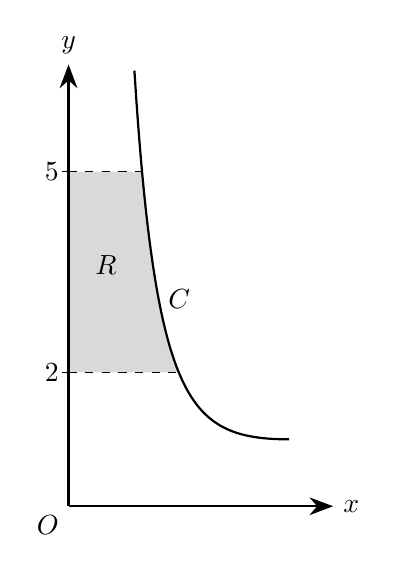
\begin{tikzpicture}[x=1.4cm,y=0.85cm]
\def\ylo{2}
\def\yhi{5}
\def\paramlo{1}
\def\paramhi{2}
\def\xmax{2.4}
\def\ymax{6.6}
\pgfmathsetmacro{\xlo}{2/(1+\paramlo)}
\pgfmathsetmacro{\xhi}{2/(1+\paramhi)}

\fill[gray!30] (0,\ylo) -- (0,\yhi) --
  plot[domain=\paramhi:\paramlo, samples=200, variable=\param] ({2/(1+\param)}, {\param*\param+1}) -- cycle;

\draw[thick, -{Stealth[length=3mm]}] (0,0) -- (\xmax,0) node[right] {$x$};
\draw[thick, -{Stealth[length=3mm]}] (0,0) -- (0,\ymax) node[above] {$y$};

\draw[dashed] (0,\ylo) -- (\xlo,\ylo);
\draw[dashed] (0,\yhi) -- (\xhi,\yhi);

\draw[thick, domain=0:2.35, samples=200, variable=\param]
  plot ({2/(1+\param)}, {\param*\param+1});

\draw (-0.06,\ylo) -- (0.06,\ylo);
\draw (-0.06,\yhi) -- (0.06,\yhi);
\node[left] at (0,\ylo) {$2$};
\node[left] at (0,\yhi) {$5$};
\node[below left] at (0,0) {$O$};

\node at (0.34,3.6) {$R$};
\coordinate (Pc) at ({2/(1+1.45)}, {1.45*1.45+1});
\node[right] at (Pc) {$C$};
\end{tikzpicture}
\end{figure}


The diagram shows part of the curve $C$ with parametric equations \[x=\frac{2}{1+t},\quad y=t^2+1,\qquad t\geq 0\]

The region $R$ is bounded by the curve, the $y$-axis and the lines $y=2$ and $y=5$. Region $R$ is rotated through $2\pi$ radians about the $y$-axis. \\

Use parametric integration to find the volume of the resulting solid of revolution. \marks{6} \\

\vspace*{10pt}

\begin{tcolorbox}[colback=white, colframe=scarlet, title={\textbf{Solution}}, breakable, grow to left by=6mm, grow to right by=10mm]
For the given curve,
\[
x=\frac{2}{1+t}, \qquad y=t^2+1, \qquad t\ge 0
\]

First find the values of $t$ corresponding to the horizontal boundaries.

When $y=2$,
\[
t^2+1=2 \implies t^2=1 \implies t=1
\]
since $t\ge 0$.

When $y=5$,
\[
t^2+1=5 \implies t^2=4 \implies t=2
\]

So the required part of the curve corresponds to $1\le t\le 2$.

When the region is rotated about the $y$-axis, the volume is
\[
V=\pi \int x^2\,\mathrm{d}y
\]

Using the parameter $t$,
\[
V=\pi \int_{1}^{2} x^2\frac{\mathrm{d}y}{\mathrm{d}t}\,\mathrm{d}t
\]

Now
\[
x^2=\left(\frac{2}{1+t}\right)^2=\frac{4}{(1+t)^2}
\]
and
\[
\frac{\mathrm{d}y}{\mathrm{d}t}=2t
\]

Hence
\[
V=\pi \int_{1}^{2}\frac{4}{(1+t)^2}\cdot 2t\,\mathrm{d}t
=8\pi \int_{1}^{2}\frac{t}{(1+t)^2}\,\mathrm{d}t
\]

Now simplify the integrand:
\[
\frac{t}{(1+t)^2}=\frac{(1+t)-1}{(1+t)^2}
=\frac{1}{1+t}-\frac{1}{(1+t)^2}
\]

So
\[
V=8\pi \int_{1}^{2}\left(\frac{1}{1+t}-\frac{1}{(1+t)^2}\right)\mathrm{d}t
\]

Integrating,
\[
\int \frac{1}{1+t}\,\mathrm{d}t=\ln(1+t)
\]
and
\[
\int -\frac{1}{(1+t)^2}\,\mathrm{d}t=\frac{1}{1+t}
\]

Therefore
\[
V=8\pi \left[\ln(1+t)+\frac{1}{1+t}\right]_{1}^{2}
\]

Substituting the limits,
\[
V=8\pi \left(\ln 3+\frac13-\ln 2-\frac12\right)
\]

So
\[
V=8\pi \left(\ln\frac32-\frac16\right)
\]
\[
V=8\pi\ln\frac32-\frac{4\pi}{3}
\]

Hence the volume of the solid is
\[
\boxed{8\pi\ln\frac32-\frac{4\pi}{3}}
\]

In decimal form,
\[
V\approx 6.00
\]
\end{tcolorbox}


\newpage

% ---- Question 12 ----
\questionitem

\begin{figure}[H]
    \centering
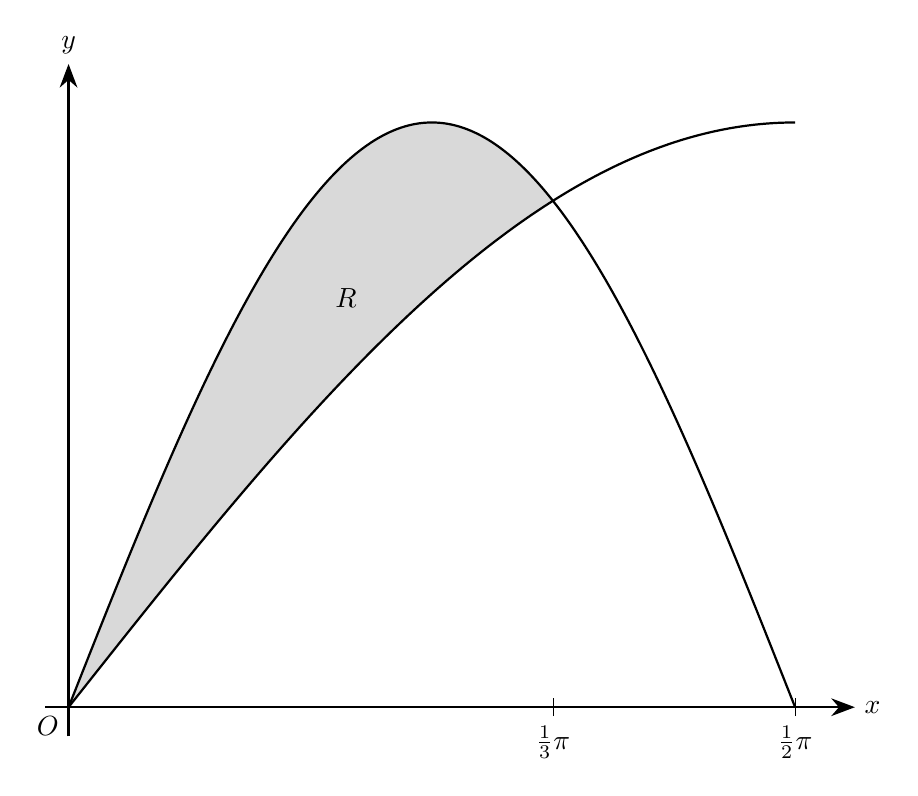
\begin{tikzpicture}[scale=1.5]
\def\halfpi{1.57079632679}
\def\thirdpi{1.04719755120}
\begin{axis}[
    axis lines=center,
    xlabel={$x$},
    ylabel={$y$},
    xmin=-0.05, xmax=1.7,
    ymin=-0.05, ymax=1.1,
    xtick={\thirdpi,\halfpi},
    xticklabels={$\frac{1}{3}\pi$,$\frac{1}{2}\pi$},
    ytick=\empty,
    clip=false,
    enlargelimits=false,
    axis line style={thick, black, -{Stealth[length=3mm]}},
    tick style={black},
    every axis x label/.style={at={(ticklabel* cs:1)}, anchor=west},
    every axis y label/.style={at={(ticklabel* cs:1)}, anchor=south}
]
\addplot[name path=sinx, thick, black, samples=200, domain=0:\halfpi] {sin(deg(x))};
\addplot[name path=sin2x, thick, black, samples=200, domain=0:\halfpi] {sin(deg(2*x))};
\addplot[gray!30] fill between[of=sin2x and sinx, soft clip={domain=0:\thirdpi}];
\node[below left] at (axis cs:0,0) {$O$};
\node at (axis cs:0.6,0.7) {$R$};
\end{axis}
\end{tikzpicture}
\end{figure}


The diagram shows the curves $y = \sin x$ and $y = \sin 2x$, for $0 \leq x \leq \frac{1}{2}\pi$. The shaded region $R$ is the finite region enclosed by the curves. \\

Find the volume of the solid of revolution formed when $R$ is rotated completely about the $x$-axis, giving your answer in terms of $\pi$. \marks{7} \\

\vspace*{10pt}

\begin{tcolorbox}[colback=white, colframe=scarlet, title={\textbf{Solution}}, breakable, grow to left by=6mm, grow to right by=10mm]
First find where the curves meet.

\[
\sin x=\sin 2x
\]

Using \(\sin 2x=2\sin x\cos x\),

\[
\sin x=2\sin x\cos x
\]

\[
\sin x(2\cos x-1)=0
\]

So, for \(0\le x\le \frac{\pi}{2}\),

\[
\sin x=0 \Rightarrow x=0
\qquad \text{or} \qquad
2\cos x-1=0 \Rightarrow \cos x=\frac12 \Rightarrow x=\frac{\pi}{3}
\]

Hence the shaded region is between \(x=0\) and \(x=\frac{\pi}{3}\).

For \(0<x<\frac{\pi}{3}\), we have \(\sin x>0\) and \(\cos x>\frac12\), so \(2\cos x-1>0\). Therefore

\[
\sin x(2\cos x-1)>0
\]

which means

\[
\sin 2x>\sin x
\]

So when the region is rotated about the \(x\)-axis, the volume is

\[
V=\pi\int_0^{\pi/3}\left((\sin 2x)^2-(\sin x)^2\right)\,\mathrm{d}x
\]

Now use

\[
\sin^2\theta=\frac{1-\cos 2\theta}{2}
\]

Then

\begin{align*}
\sin^2 2x-\sin^2 x
&=\frac{1-\cos 4x}{2}-\frac{1-\cos 2x}{2}\\
&=\frac{\cos 2x-\cos 4x}{2}
\end{align*}

So

\begin{align*}
V
&=\pi\int_0^{\pi/3}\frac{\cos 2x-\cos 4x}{2}\,\mathrm{d}x\\
&=\pi\left[\frac{\sin 2x}{4}-\frac{\sin 4x}{8}\right]_0^{\pi/3}
\end{align*}

Now substitute the limits:

\begin{align*}
V
&=\pi\left(\frac{\sin(2\pi/3)}{4}-\frac{\sin(4\pi/3)}{8}\right)\\
&=\pi\left(\frac{\sqrt3/2}{4}-\frac{-\sqrt3/2}{8}\right)\\
&=\pi\left(\frac{\sqrt3}{8}+\frac{\sqrt3}{16}\right)\\
&=\frac{3\sqrt3\pi}{16}
\end{align*}

The volume of the solid of revolution is \(\displaystyle \frac{3\sqrt3\pi}{16}\).
\end{tcolorbox}


\newpage

% ---- Question 13 ----
\questionitem

\begin{figure}[H]
    \centering
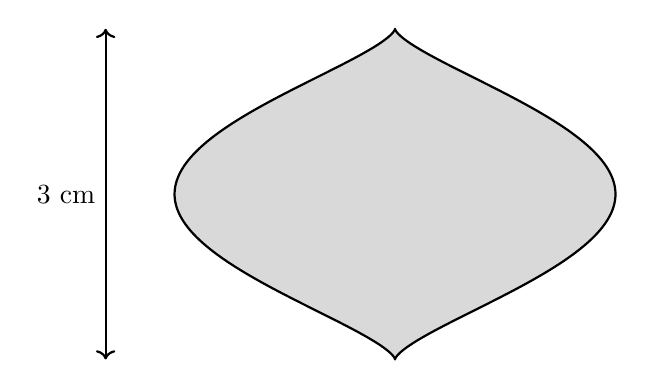
\begin{tikzpicture}[scale=2.1]
\def\dimx{-1.75}
\draw[thick, fill=gray!30, line join=round]
  plot[domain=0:360, samples=400, variable=\t]
    ({sin(\t) - (1/3)*sin(3*\t)}, {1 - cos(\t)})
  -- cycle;
\draw[<->, thick] (\dimx, 0) -- (\dimx, 2)
  node[midway, left] {$3\ \mathrm{cm}$};
\end{tikzpicture}
\end{figure}


The diagram shows the outline of a glass bead. The bead is modelled by the solid obtained when the region enclosed by a curve $C$ is rotated about the $y$-axis. The actual bead has height $3\ \mathrm{cm}$. The curve $C$ has parametric equations
\[
x = \sin\theta - \frac{1}{3}\sin 3\theta,\qquad y = 1 - \cos\theta,\qquad 0 \le \theta \le 2\pi
\] \\

\begin{enumerate}[label=\textbf{(\alph*)}]
  \item Show that a Cartesian equation of the curve $C$ is
  \[
  x^2 = \frac{16}{9}y^3(2-y)^3
  \]
  \marks[-20pt]{4}
  \item Hence, using the model, find, in $\mathrm{cm}^3$, the volume of the bead. \marks{5} \\
\end{enumerate}

\vspace*{10pt}

\begin{tcolorbox}[colback=white, colframe=scarlet, title={\textbf{Solution}}, breakable, grow to left by=6mm, grow to right by=10mm]
\begin{enumerate}[label=\textbf{(\alph*)}]
  \item Using the identity
\[
\sin 3\theta = 3\sin\theta - 4\sin^3\theta
\]
we have
\begin{align*}
x&=\sin\theta-\frac13\sin 3\theta\\
&=\sin\theta-\frac13\left(3\sin\theta-4\sin^3\theta\right)\\
&=\sin\theta-\sin\theta+\frac43\sin^3\theta\\
&=\frac43\sin^3\theta
\end{align*}
So
\[
x^2=\frac{16}{9}\sin^6\theta
\]

Also
\[
y=1-\cos\theta
\]
so
\[
\cos\theta=1-y
\]
Hence
\begin{align*}
\sin^2\theta&=1-\cos^2\theta\\
&=1-(1-y)^2\\
&=1-(1-2y+y^2)\\
&=2y-y^2\\
&=y(2-y)
\end{align*}
Therefore
\[
\sin^6\theta=\left(\sin^2\theta\right)^3=\left(y(2-y)\right)^3
\]
and so
\begin{align*}
x^2&=\frac{16}{9}\sin^6\theta\\
&=\frac{16}{9}\left(y(2-y)\right)^3\\
&=\frac{16}{9}y^3(2-y)^3
\end{align*}

Thus a Cartesian equation of $C$ is
\[
x^2=\frac{16}{9}y^3(2-y)^3
\]

  \item The model has height
\[
2-0=2
\]
whereas the actual bead has height $3\text{ cm}$, so the linear scale factor is
\[
k=\frac32
\]

First find the volume of the model.

When the region is rotated about the $y$-axis,
\[
V_{\text{model}}=\pi\int_0^2 x^2\,\mathrm{d}y
\]
Using the result from part (a),
\begin{align*}
V_{\text{model}}&=\pi\int_0^2 \frac{16}{9}y^3(2-y)^3\,\mathrm{d}y\\
&=\frac{16\pi}{9}\int_0^2 y^3(2-y)^3\,\mathrm{d}y
\end{align*}
Now expand:
\begin{align*}
(2-y)^3&=8-12y+6y^2-y^3\\
y^3(2-y)^3&=8y^3-12y^4+6y^5-y^6
\end{align*}
So
\begin{align*}
V_{\text{model}}
&=\frac{16\pi}{9}\int_0^2 \left(8y^3-12y^4+6y^5-y^6\right)\,\mathrm{d}y\\
&=\frac{16\pi}{9}\left[2y^4-\frac{12}{5}y^5+y^6-\frac17 y^7\right]_0^2
\end{align*}
Substituting the limits,
\begin{align*}
V_{\text{model}}
&=\frac{16\pi}{9}\left(2(2^4)-\frac{12}{5}(2^5)+2^6-\frac17(2^7)\right)\\
&=\frac{16\pi}{9}\left(32-\frac{384}{5}+64-\frac{128}{7}\right)\\
&=\frac{16\pi}{9}\cdot \frac{32}{35}\\
&=\frac{512\pi}{315}
\end{align*}

Volume scales as the cube of the linear scale factor, so
\begin{align*}
V_{\text{actual}}
&=\left(\frac32\right)^3 V_{\text{model}}\\
&=\frac{27}{8}\times \frac{512\pi}{315}\\
&=\frac{192\pi}{35}
\end{align*}

Therefore the volume of the bead is
\[
\frac{192\pi}{35}\ \mathrm{cm}^3 \approx 17.2\ \mathrm{cm}^3
\]
\end{enumerate}
\end{tcolorbox}

\newpage
% ---- Question 14 ----
\questionitem

The equation of a curve is \[y=\frac{x}{\sqrt{k^2+x^2}}\] where $k$ is a positive constant. \\

The region in the first quadrant bounded by the curve, the $x$-axis, the $y$-axis and the line $x=k$ is rotated through $2\pi$ radians about the $x$-axis

Given that the volume of revolution formed is $1\text{ unit}^3$, find the exact value of $k$ \marks{4} \vspace*{20pt}

\begin{tcolorbox}[colback=white, colframe=scarlet, title={\textbf{Solution}}, breakable, grow to left by=6mm, grow to right by=10mm]
When the region is rotated about the $x$-axis, the volume is
\[
V=\pi\int_0^k y^2\,\mathrm{d}x
\]

Here
\[
y=\frac{x}{\sqrt{k^2+x^2}}
\qquad\Rightarrow\qquad
y^2=\frac{x^2}{k^2+x^2}
\]

So
\[
V=\pi\int_0^k \frac{x^2}{k^2+x^2}\,\mathrm{d}x
\]

Rewrite the integrand:
\[
\frac{x^2}{k^2+x^2}
=\frac{k^2+x^2-k^2}{k^2+x^2}
=1-\frac{k^2}{k^2+x^2}
\]

Hence
\[
V=\pi\int_0^k \left(1-\frac{k^2}{k^2+x^2}\right)\,\mathrm{d}x
\]

Now integrate:
\begin{align*}
\int \left(1-\frac{k^2}{k^2+x^2}\right)\,\mathrm{d}x
&=x-k^2\int \frac{1}{k^2+x^2}\,\mathrm{d}x \\
&=x-k^2\left(\frac{1}{k}\arctan\frac{x}{k}\right) \\
&=x-k\arctan\frac{x}{k}
\end{align*}

Therefore
\begin{align*}
V
&=\pi\left[x-k\arctan\frac{x}{k}\right]_0^k \\
&=\pi\left(k-k\arctan 1\right) \\
&=\pi\left(k-k\cdot\frac{\pi}{4}\right) \\
&=\pi k\left(1-\frac{\pi}{4}\right)
\end{align*}

We are given that the volume is $1$, so
\[
\pi k\left(1-\frac{\pi}{4}\right)=1
\]

Solving for $k$:
\begin{align*}
k
&=\frac{1}{\pi\left(1-\frac{\pi}{4}\right)} \\
&=\frac{1}{\pi\left(\frac{4-\pi}{4}\right)} \\
&=\frac{4}{\pi(4-\pi)}
\end{align*}

Since $k$ is positive, this is valid.

The exact value of $k$ is
\[
k=\frac{4}{\pi(4-\pi)}
\]
\end{tcolorbox}


\newpage

% ---- Question 15 ----
\questionitem

\begin{enumerate}[label=\textbf{(\alph*)}]
  \item Prove that
  \[
  \cos 4\theta \cos \theta \equiv \frac{1}{2}(\cos 5\theta + \cos 3\theta)
  \]
  \marks[-20pt]{3}
\end{enumerate}

\begin{figure}[H]
    \centering
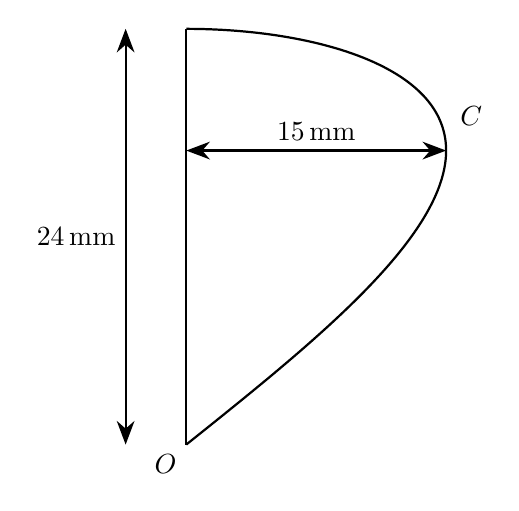
\begin{tikzpicture}[scale=1.1]
\def\a{3}
\def\b{4.8}
\pgfmathsetmacro{\ymid}{\b/sqrt(2)}

\coordinate (O) at (0,0);
\coordinate (T) at (0,\b);
\coordinate (A) at (0,\ymid);
\coordinate (W) at (\a,\ymid);
\coordinate (H1) at (-0.7,0);
\coordinate (H2) at (-0.7,\b);

\draw[thick] (O) -- (T);
\draw[thick, domain=0:90, samples=200] plot ({\a*sin(2*\x)}, {\b*sin(\x)});

\draw[{Stealth[length=3mm]}-{Stealth[length=3mm]}, thick] (H1) -- (H2) node[midway, left] {$24\,\mathrm{mm}$};
\draw[{Stealth[length=3mm]}-{Stealth[length=3mm]}, thick] (A) -- (W) node[midway, above] {$15\,\mathrm{mm}$};

\node[below left] at (O) {$O$};
\node[right] at ($(W)+(0.05,0.4)$) {$C$};
\end{tikzpicture}
\end{figure}


The diagram shows the cross-section of a decorative ornament. \\

The ornament can be modelled by rotating the region enclosed by the curve $C$ and the $y$-axis about the $y$-axis. Curve $C$ has parametric equations
\[
x = 15\sin 2\theta, \quad y = 24\sin \theta, \quad 0 \leq \theta \leq \frac{\pi}{2}
\]
where $x$ and $y$ are measured in millimetres. \\
\begin{enumerate}[label=\textbf{(\alph*)}, resume]
  \item Find the volume of the ornament. \marks{5} \\
\end{enumerate}

\vspace*{10pt}

\begin{tcolorbox}[colback=white, colframe=scarlet, title={\textbf{Solution}}, breakable, grow to left by=6mm, grow to right by=10mm]
\begin{enumerate}[label=\textbf{(\alph*)}]
  \item Using the cosine addition formula,
\[
\cos 5\theta=\cos(4\theta+\theta)=\cos 4\theta\cos\theta-\sin 4\theta\sin\theta
\]
and
\[
\cos 3\theta=\cos(4\theta-\theta)=\cos 4\theta\cos\theta+\sin 4\theta\sin\theta
\]

Adding these gives
\begin{align*}
\cos 5\theta+\cos 3\theta
&=(\cos 4\theta\cos\theta-\sin 4\theta\sin\theta)
+(\cos 4\theta\cos\theta+\sin 4\theta\sin\theta)\\
&=2\cos 4\theta\cos\theta
\end{align*}

Therefore
\[
\cos 4\theta\cos\theta \equiv \frac12(\cos 5\theta+\cos 3\theta)
\]

So the required identity is proved.

  \item When the region is rotated about the $y$-axis, the volume is
\[
V=\pi\int x^2\,\mathrm{d}y
\]

Using the parameter $\theta$,
\[
V=\pi\int_0^{\pi/2}x^2\frac{\mathrm{d}y}{\mathrm{d}\theta}\,\mathrm{d}\theta
\]

Now
\[
x=15\sin 2\theta,\qquad y=24\sin\theta
\]
so
\[
\frac{\mathrm{d}y}{\mathrm{d}\theta}=24\cos\theta
\]

Substituting,
\begin{align*}
V&=\pi\int_0^{\pi/2}(15\sin 2\theta)^2(24\cos\theta)\,\mathrm{d}\theta\\
&=5400\pi\int_0^{\pi/2}\sin^2 2\theta\cos\theta\,\mathrm{d}\theta
\end{align*}

Use
\[
\sin^2 2\theta=\frac{1-\cos 4\theta}{2}
\]

Then
\begin{align*}
V&=5400\pi\int_0^{\pi/2}\frac{1-\cos 4\theta}{2}\cos\theta\,\mathrm{d}\theta\\
&=2700\pi\int_0^{\pi/2}(1-\cos 4\theta)\cos\theta\,\mathrm{d}\theta\\
&=2700\pi\left(\int_0^{\pi/2}\cos\theta\,\mathrm{d}\theta-\int_0^{\pi/2}\cos 4\theta\cos\theta\,\mathrm{d}\theta\right)
\end{align*}

From part (a),
\[
\cos 4\theta\cos\theta=\frac12(\cos 5\theta+\cos 3\theta)
\]

So
\begin{align*}
V&=2700\pi\int_0^{\pi/2}\left(\cos\theta-\frac12(\cos 5\theta+\cos 3\theta)\right)\,\mathrm{d}\theta\\
&=2700\pi\left[\sin\theta-\frac{1}{10}\sin 5\theta-\frac{1}{6}\sin 3\theta\right]_0^{\pi/2}
\end{align*}

Now evaluate the bracket:
\[
\sin\frac{\pi}{2}=1,\qquad \sin\frac{5\pi}{2}=1,\qquad \sin\frac{3\pi}{2}=-1
\]

Hence
\begin{align*}
V&=2700\pi\left(1-\frac{1}{10}-\frac{1}{6}(-1)\right)\\
&=2700\pi\left(1-\frac{1}{10}+\frac{1}{6}\right)\\
&=2700\pi\left(\frac{16}{15}\right)\\
&=2880\pi
\end{align*}

Therefore the volume of the ornament is
\[
2880\pi\ \text{mm}^3
\]

which is approximately
\[
9.05\times 10^3\ \text{mm}^3
\]
  \end{enumerate}
\end{tcolorbox}


\end{enumerate}
\end{document}
